\documentclass[14pt,a4paper,report]{report}
\usepackage[a4paper, mag=1000, left=2.5cm, right=1cm, top=2cm, bottom=2cm, headsep=0.7cm, footskip=1cm]{geometry}
\usepackage[utf8]{inputenc}
\usepackage[english,russian]{babel}
\usepackage{indentfirst}
\usepackage[dvipsnames]{xcolor}
\usepackage[colorlinks]{hyperref}
\usepackage{listings} 
\usepackage{fancyhdr}
\usepackage{caption}
\usepackage{amsmath}
\usepackage{graphicx}
\usepackage{amsmath}
\usepackage{booktabs}
\usepackage{array}
\newcolumntype{P}[1]{>{\centering\arraybackslash}p{#1}}
\hypersetup{
	colorlinks = true,
	linkcolor  = black
}

\usepackage{titlesec}
\titleformat{\chapter}
{\Large\bfseries} % format
{}                % label
{0pt}             % sep
{\huge}           % before-code


\DeclareCaptionFont{white}{\color{white}} 

% Listing description
\usepackage{listings} 
\DeclareCaptionFormat{listing}{\colorbox{gray}{\parbox{\textwidth}{#1#2#3}}}
\captionsetup[lstlisting]{format=listing,labelfont=white,textfont=white}
\lstset{ 
	% Listing settings
	inputencoding = utf8,			
	extendedchars = \true, 
	keepspaces = true, 			  	 % Поддержка кириллицы и пробелов в комментариях
	language = Prolog,            	 	 % Язык программирования (для подсветки)
	basicstyle = \small\sffamily, 	 % Размер и начертание шрифта для подсветки кода
	numbers = left,               	 % Где поставить нумерацию строк (слева\справа)
	numberstyle = \tiny,          	 % Размер шрифта для номеров строк
	stepnumber = 1,               	 % Размер шага между двумя номерами строк
	numbersep = 5pt,              	 % Как далеко отстоят номера строк от подсвечиваемого кода
	backgroundcolor = \color{white}, % Цвет фона подсветки - используем \usepackage{color}
	showspaces = false,           	 % Показывать или нет пробелы специальными отступами
	showstringspaces = false,    	 % Показывать или нет пробелы в строках
	showtabs = false,           	 % Показывать или нет табуляцию в строках
	frame = single,              	 % Рисовать рамку вокруг кода
	tabsize = 2,                  	 % Размер табуляции по умолчанию равен 2 пробелам
	captionpos = t,             	 % Позиция заголовка вверху [t] или внизу [b] 
	breaklines = true,           	 % Автоматически переносить строки (да\нет)
	breakatwhitespace = false,   	 % Переносить строки только если есть пробел
	escapeinside = {\%*}{*)}      	 % Если нужно добавить комментарии в коде
}

\begin{document}

\def\contentsname{Содержание}

% Titlepage
\begin{titlepage}
	\begin{center}
		\textsc{Санкт-Петербургский Политехнический 
			Университет Петра Великого\\[5mm]
			Кафедра компьютерных систем и программных технологий}
		
		\vfill
		
		\textbf{Отчёт по лабораторной работе №5\\[3mm]
			Курс: «Многоагентные системы»\\[41mm]
		}
	\end{center}
	
	\hfill
	\begin{minipage}{.4\textwidth}
		Выполнил студент:\\[2mm] 
		Бояркин Н.С.\\
		Группа: 13541/3\\[5mm]
		
		Проверил:\\[2mm] 
		Сазанов А.М.
	\end{minipage}
	\vfill
	\begin{center}
		Санкт-Петербург\\ \the\year\ г.
	\end{center}
\end{titlepage}

% Contents
\tableofcontents
\clearpage

\chapter{Лабораторная работа №5}

\section{Цель работы}

Познакомиться с принципами работы многоагентных систем, а также изучить основные возможности основных платформ для разработки таких систем.

\section{Программа работы}

\begin{enumerate}
	\item Дайте определение и краткую классификацию многоагентных интеллектуальных систем.	В чем преимущества и в чем недостатки многоагентного подхода?
	\item Приведите наиболее полную классификацию таких систем, кратко поясните по какому признаку дана эта классификация.
	\item Какие задачи решаются с помощью многоагентного подхода. Приведите не менее ДВУХ примеров задач, с кратким описанием.
	\item Проанализируйте преимущества и недостатки многоагентного подхода на примере задач из предыдущего пункта. Сформулируйте общие проблемы \textbackslash недостатки и общие преимущества \textbackslash достоинства такого подхода.
	\item Проанализировать основные платформы для разработки многоагентных систем: выбрать одну из платформ (Например, NetLogo, StarLogo, Repast Simphony, Eclipse AMP, JADE, Jason либо другую) и провести обзор основных функциональных возможностей:
	\begin{itemize}
		\item Процесс установки ПО, ссылки на сайты ссылки на необходимы драйвера и т.д. (если нужно)
		\item Процесс создания простого проекта.
		\item Анализ одного примера (ссылка на пример, описание алгоритма работы и процесса моделирования и т.д.)
		\item Опишите основные возможности данного ПО применительно для создания многоагентных систем. Опишите замеченные недостатки или наоборот опишите достоинства данного ПО.
	\end{itemize}
	\item Написать выводы. В выводах отразить, помимо своих мыслей, возникших в ходе работы, ответы на приведенные ниже вопросы:
	\begin{itemize}
		\item В чем Плюсы и минусы многоагентного подхода?
		\item Какие еще среды или языки программирования использует для создания многоагентных систем?
		\item Как по-вашему стоит ли развивать данное направление, если нет, то почему, если да, то в какую сторону?
		\item Корректно ли по-вашему моделирование многоагентных систем на одной вычислительной машине (рассмотреть два варианта, итеративный перебор агентом в цикле, и создание для каждого агента своего процесса)
		\item Приведите области \textbackslash примеры в которых применение многоагентного подхода дает максимально положительные результаты.
	\end{itemize}
\end{enumerate}

\clearpage

\section{Ход работы}

\subsection{Определение и краткая классификация многоагентных интеллектуальных систем. Преимущества и в чем недостатки многоагентного подхода.}

\textbf{Многоагентные системы} – это направление искусственного интеллекта, которое для решения сложной задачи или проблемы использует системы, состоящие из множества взаимодействующих агентов [1]

\textbf{Агент} — это аппаратная или программная сущность, способная действовать в интересах достижения целей, поставленных пользователем. Агенты описываются рядом свойств, которые характеризуют понятие агента:

\begin{itemize}
	\item \textbf{Автономность} -- способность функционировать без прямого вмешательства людей или компьютерных средств и при этом осуществлять самоконтроль над своими действиями и внутренними состояниями;
	\item \textbf{Реактивность} -- способность  воспринимать состояние среды  (физического мира, пользователя – через пользовательский  интерфейс, совокупности других агентов, сети Internet, или сразу все этих компонентов внешней среды);
	\item \textbf{Активность} -- способность агентов не просто реагировать на стимулы, поступающие из среды, но и осуществлять целенаправленное поведение, проявляя инициативу.
\end{itemize}

В отличие от классической теории искусственного интеллекта, где агент (ИС) имеет в своем распоряжении все необходимые данные и вычислительные ресурсы, в теории многоагентных систем один агент владеет всего лишь частичным представлением о глобальной проблеме, а значит, он может решить лишь некоторую часть общей задачи.

\subsubsection{Общая классификация агентов}

В наиболее общем смысле, многоагентные системы принято различать по их архитектуре:

\begin{itemize}
	\item \textbf{Делиберативная архитектура} -- Подход на основе символьной модели мира, в которой решения принимаются путем логических рассуждений. Такие агенты называются агентами, основанными на знаниях. Для представления знаний используются хорошо известные в системах искусственного интеллекта методы - логический, продукционный, семантический, фреймовый [2]
	\item \textbf{Реактивная архитектура} -- Подход основывается на том, что интеллектуальное поведение может быть обеспечено без использования символьной модели мира, путем формирования реакций агента на события внешнего мира [2]
	\item \textbf{Гибридная архитектура} -- объединяет преимущества как делиберативной, так и реактивной архитектур.
\end{itemize}

Кроме того, в качестве общей классификации многоагентных систем следует выделить области, в которых эти системы применяются:

\begin{figure}[h!]
	\centering
	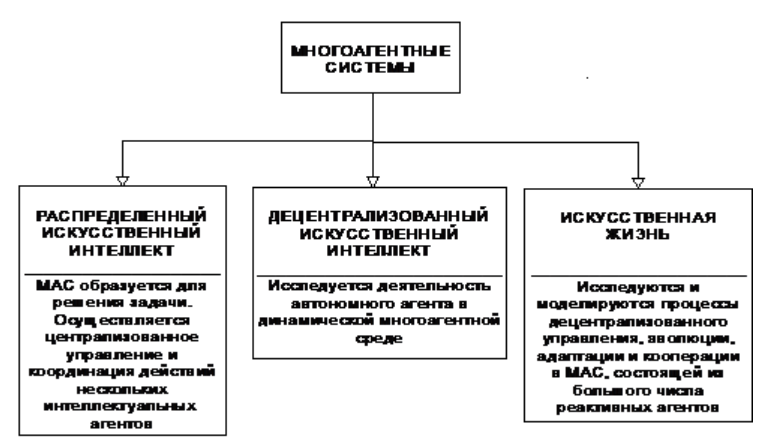
\includegraphics[scale = 0.57]{images/0_0.png}
	\caption{Классификация многоагентных систем по областям применения [3]}
\end{figure}

\subsubsection{Преимущества и в чем недостатки многоагентного подхода}

Основные преимущества использования многоагентных систем, это: \textbf{распределенные вычисления}, \textbf{масштабирование} и \textbf{автономность}. Кроме того агенты могут общаться между собой, обмениваться информацией и кооперироваться для выполнения задач.

Из недостатков следует выделить усложнение структуры за счет количества агентов, что впоследствии ведет к \textbf{плохой наблюдаемости} и \textbf{непредсказуемости} системы.

\subsection{Приведите наиболее полную классификацию таких систем, кратко поясните по какому признаку дана эта классификация.}

Приведем наиболее подробную классификацию агентов:

\begin{figure}[h!]
	\centering
	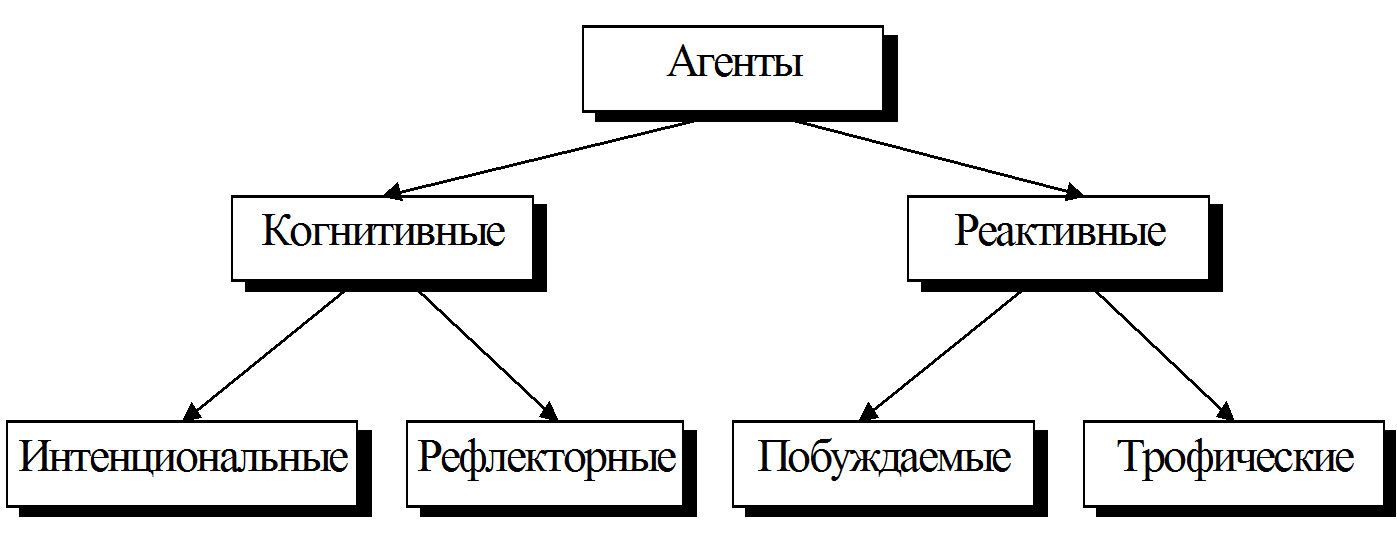
\includegraphics[scale = 0.37]{images/0_1.png}
	\caption{Классификация агентов}
\end{figure}

\textbf{Интеллектуальные агенты} обладают хорошо развитой и пополняемой символьной моделью внешнего мира, что достигается благодаря наличию у них базы знаний, механизмов решения и анализа действий. Небольшое различие между этими типами интеллектуальных агентов связано с расстановкой акцентов на тех или иных интеллектуальных функциях: либо на получении знаний о среде, либо на рассуждениях о возможных действиях. У коммуникативных агентов внутренняя модель мира превращается главным образом в модель общения, состоящую из моделей участников, процесса и желаемого результата общения. Наконец, база знаний ресурсного агента содержит в основном знания о структуре и состоянии ресурсов, определяющих различные формы поведения [5]

Далее, по типу поведения интеллектуальные агенты делятся на \textbf{интенциональных} и \textbf{рефлекторных}. Большинство интеллектуальных (когнитивных) агентов можно отнести к числу интенциональных. Подобные агенты наделены собственными механизмами мотивации. Это означает, что в них так или иначе моделируются внутренние убеждения, желания, намерения и мотивы, порождающие цели, которые и определяют их действия. В свою очередь, модульные или рефлекторные агенты не имеют внутренних источников мотивации и собственных целей, а их поведение характеризуется простейшими (одношаговыми) выводами или автоматизмами [5]

\textbf{Реактивные агенты} не имеют ни сколько-нибудь развитого представления внешней среды, ни механизма многошаговых рассуждений, ни достаточного количества собственных ресурсов. Отсюда вытекает еще одно существенное различие между интеллектуальными и реактивными агентами, связанное с возможностями прогнозирования изменений внешней среды и, как следствие, своего будущего. В силу вышеуказанных недостатков реактивные агенты обладают очень ограниченным диапазоном предвидения. Они практически не способны планировать свои действия, поскольку реактивность в чистом виде означает такую структуру обратной связи, которая не содержит механизмов прогноза. Тогда как интеллектуальные агенты, благодаря богатым внутренним представлениям внешней среды и возможностям рассуждений, могут запоминать и анализировать различные ситуации, предвидеть возможные реакции на свои действия, делать из этого выводы, полезные для дальнейших действий и, в результате, планировать свое поведение [5]

По сложности этих реакций и происхождению источников мотивации реактивные агенты подразделяются на \textbf{побуждаемых} и \textbf{трофических} агентов. В случае трофических агентов поведение определяется простейшими трофическими связями. Типичной моделью подобных агентов являются клеточные автоматы, где основными параметрами выступают: радиус восприятия агента, количество условных единиц питания во внешней среде и энергетическая стоимость единицы. Между тем, побуждаемые агенты также могут иметь примитивный механизм мотивации, толкающий их на выполнение задачи, например, удовлетворение набора жизненных потребностей. Речь идет о поддержании энергетического баланса или, в более широком плане, об условиях выживания агента [5]

В соответствии с этой классификацией структурируем данные о когнитивных и реактивных агентах в виде таблицы:

\begin{figure}[h!]
	\centering
	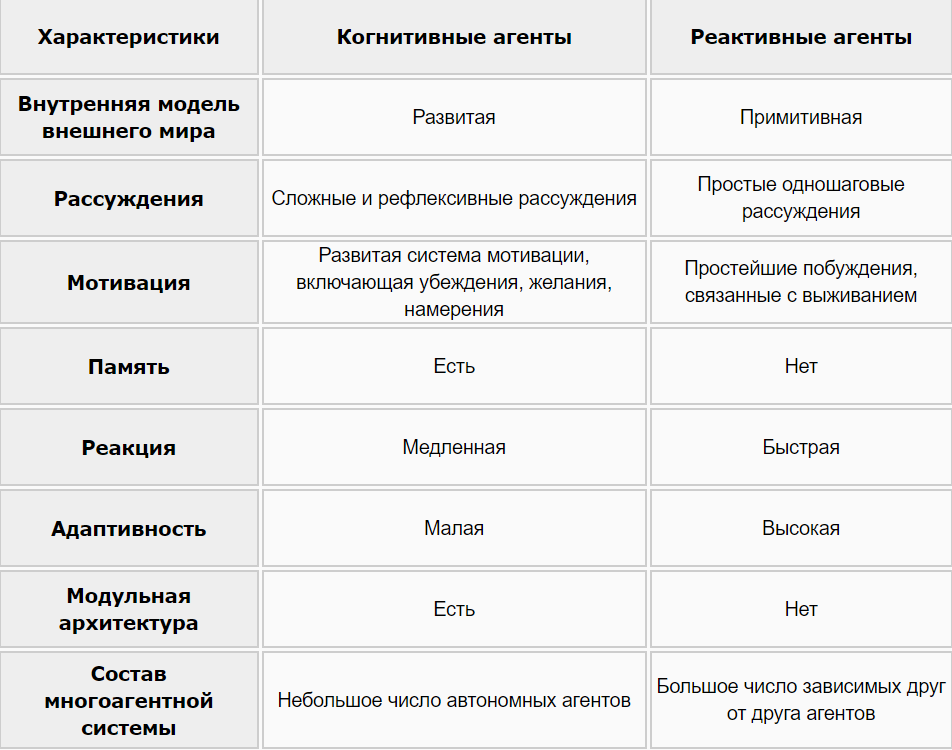
\includegraphics[scale = 0.55]{images/0_2.png}
	\caption{Сравнительная характеристика когнитивных и реактивных агентов [5]}
\end{figure}

\subsection{Какие задачи решаются с помощью многоагентного подхода. Приведите не менее ДВУХ примеров задач, с кратким описанием.}

Примеры использования многоагентных систем:

\begin{itemize}
	\item Многоагентные системы широко используются при моделировании естественнонаучных и социальных процессов с целью выявления макрозакономерностей.
	\item Многоагентные системы хорошо зарекомендовали себя в сфере сетевых и мобильных технологий, для обеспечения автоматического и динамического баланса нагруженности, расширяемости и способности к самовосстановлению.
\end{itemize}

\subsection{Проанализируйте преимущества и недостатки многоагентного подхода на примере задач из предыдущего пункта.}

Достоинства использования многоагентного подхода при моделировании естественнонаучных и социальных процессов очевидны: как правило в этих областях моделируется большое количество различных распределенных агентов (атомы, клетки, нейроны, животные, люди и т.д.), каждый из которых имеет представление только о своей задаче и может взаимодействовать с другими агентами. Таким образом все преимущества многоагентного подхода, указанные выше справедливы и для этих областей.

Из недостатков многоагентного подхода при моделировании естественнонаучных и социальных процессов следует выделить непредсказуемость этих систем, так как наращивание количества таких распределенных агентов может быть очень быстрым в зависимости от начальных критериев. 

То же самое справедливо для сферы сетевых и мобильных технологий, где количество агентов чаще всего не такое большое, но каждый из объектов обладает собственным поведением, не знает о состоянии всей системы и может взаимодействовать с другими агентами. Для данного примера не будет недостатка связанного с неконтролируемым наращиванием количества агентов, так как они чаще всего уже заданы изначально.

\subsection{Анализ системы NetLogo и обзор основных функциональных возможностей}

Среда программирования NetLogo служит для моделирования ситуаций и феноменов, происходящих в природе и обществе. NetLogo удобно использовать для моделирования сложных, развивающихся во времени систем. Создатель модели может давать указания сотням и тысячам независимых агентов действующим параллельно. Это открывает возможность для объяснения и понимания связей между поведением отдельных индивидуумов и явлениями, которые происходят на макро уровне [6]

Язык NetLogo достаточно прост и ученики и учителя могут создавать в этой среде свои собственные авторские модели. В то же время это достаточно мощный язык и среда для проведения исследовательских работ. Библиотека NetLogo содержит множество готовых моделей по биологии, математике, химии, социология. С этими моделями могут ознакомиться и поиграть ученики.

\subsubsection{Процесс установки ПО}

NetLogo распространяется бесплатно и может быть загружен с официального сайта [7] для операционных систем Windows, Linux, Mac OS. Перед скачиванием установщика предлагается заполнить следующую форму:

\begin{figure}[h!]
	\centering
	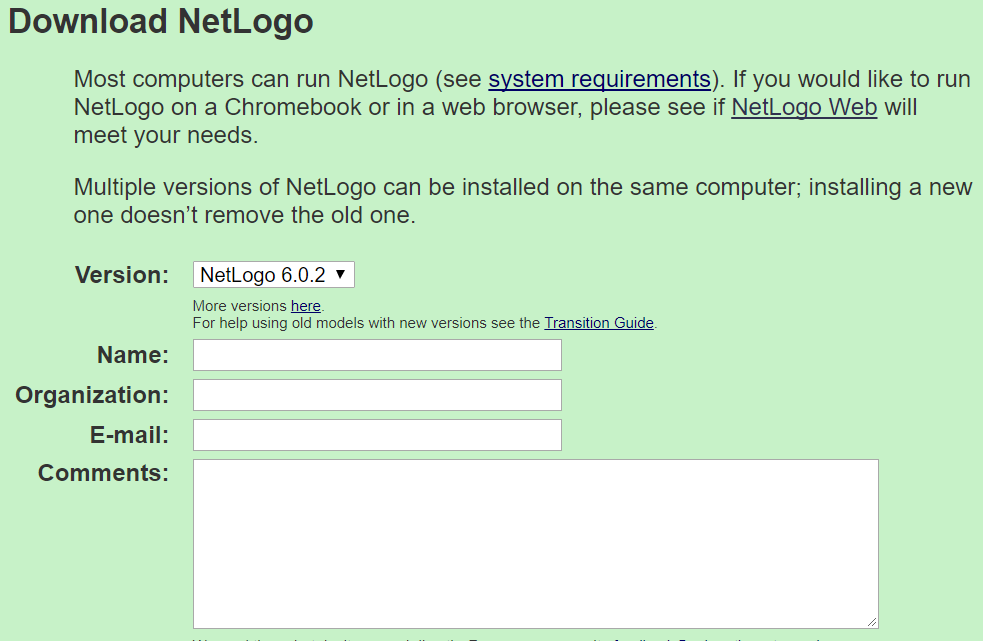
\includegraphics[scale = 0.33]{images/0_3.png}
	\caption{Форма заполнения}
\end{figure}

Дальнейший процесс установки тривиален: для Windows и Mac OS типичный файл загрузчик, а для Linux распаковываемый архив.

\subsubsection{Процесс создания простого проекта.}

Проект может быть создан или открыт комбинациями клавиш Ctrl+N, Ctrl+O соответственно или из меню приложения. Кроме того проект может быть импортирован из библиотеки демонстрационных проектов комбинацией клавиш Ctrl+M или из меню приложения.

\begin{figure}[h!]
	\centering
	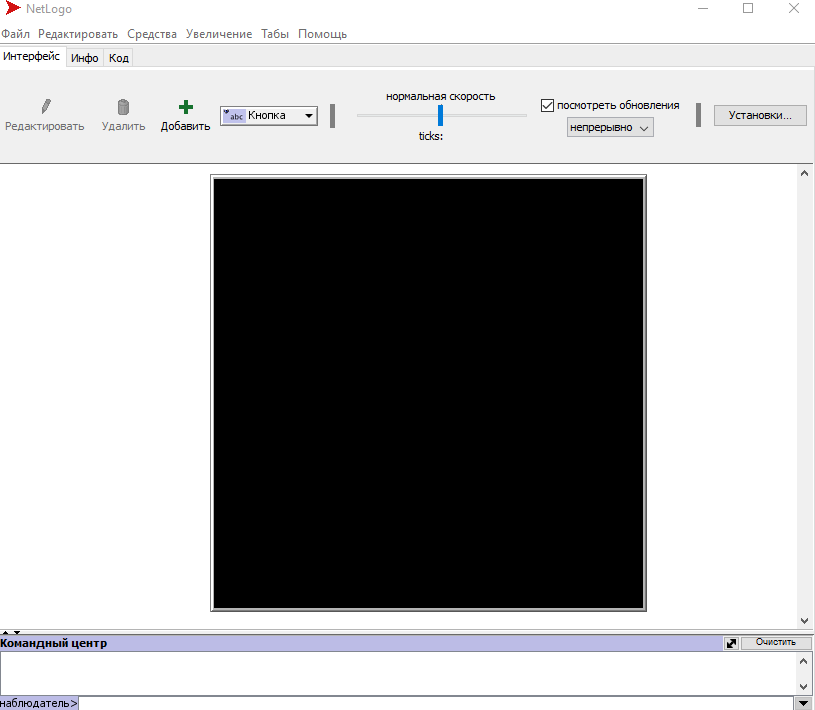
\includegraphics[scale = 0.33]{images/1.png}
	\caption{Пустой проект}
\end{figure}

После этого не нужно предпринимать каких-либо дополнительных действий и проект будет доступен для редактирования.

\subsubsection{Анализ одного примера}

В качестве примера возьмем демонстрационный проект из сферы биологии демонстрирующий популяцию волков и овец в изолированной системе. Данный проект может быть найден в библиотеке демонстрационных проектов в папке SampleModels -> Biology -> Wolf Sheep Predation.

\begin{figure}[h!]
	\centering
	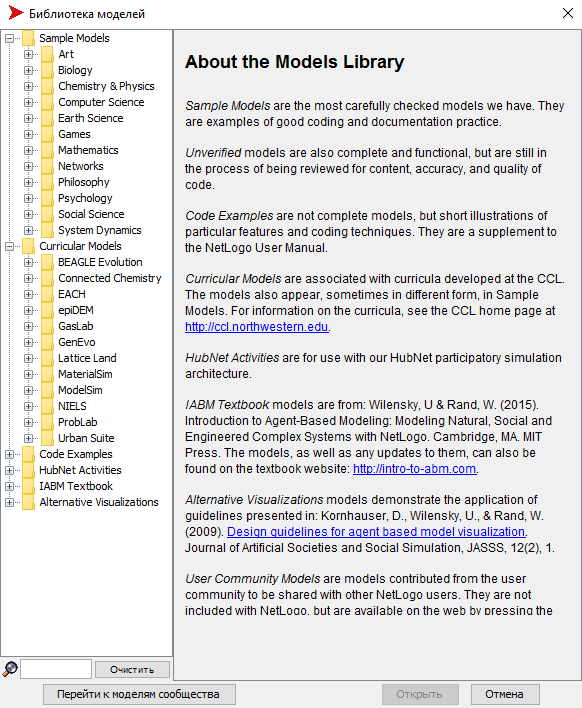
\includegraphics[scale = 0.60]{images/2.png}
	\caption{Библиотека демонстрационных проектов}
\end{figure}

Стоит отметить, что данная библиотека имеет множество примеров использования многоагентных систем во многих научных и общественных сферах: биология, химия, искусство, психология и т.д.

\begin{figure}[h!]
	\centering
	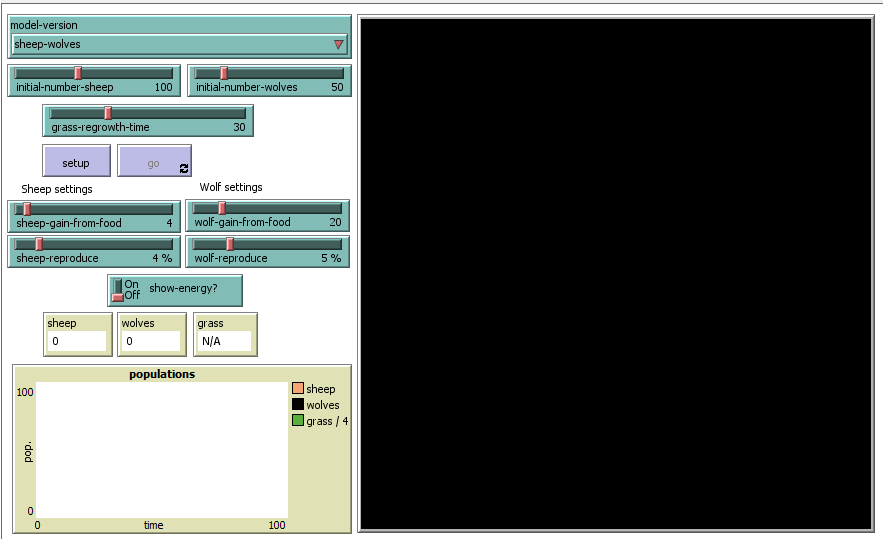
\includegraphics[scale = 0.60]{images/3.png}
	\caption{Демонстрационный проект}
\end{figure}

После загрузки проекта в глаза бросается пользовательский интерфейс. NetLogo позволяет использовать кнопки, выпадающие списки, переключатели, рычаги и текстовые поля в качестве входных данных, а также экраны, графики, метки, диалоговые окна в качестве выходных данных.

В данном демонстрационном проекте два типа агентов: волк и овца. Эти типы агентов \textbf{побуждаемые}, так как имеют примитивный организм мотивации, толкающий их на удовлетворение собственных потребностей.

Демонстрация ведется в двух режимах:

\begin{itemize}
	\item \textbf{sheep-wolfes} -- Травы нет. У волков есть показатель энергии задаваемый при инициализации, который увеличивается на заданное значение, если волк съел овцу. Показатель энергии волка уменьшается с каждым тактом и если доходит до нуля, то волк умирает. Овца умирает только если ее съел волк. Волк или овца могут с заданным шансом воспроизвести потомство.
	\item \textbf{sheep-wolfes-grass} -- Есть трава. У волков есть показатель энергии задаваемый при инициализации, который увеличивается на заданное значение, если волк съел овцу. Показатель энергии волка уменьшается с каждым тактом и если доходит до нуля, то волк умирает. Овца умирает если ее съел волк. У овец есть показатель энергии задаваемый при инициализации, который увеличивается на заданное значение, если овца съела траву. Показатель энергии овцы уменьшается с каждым тактом и если доходит до нуля, то овца умирает. Трава вырастает на клетках без травы с заданным интервалом. Волк или овца могут с заданным шансом воспроизвести потомство.
\end{itemize}

Инициализируем демонстрационный проект и запустим его в режиме sheep-wolfes:

\begin{figure}[h!]
	\centering
	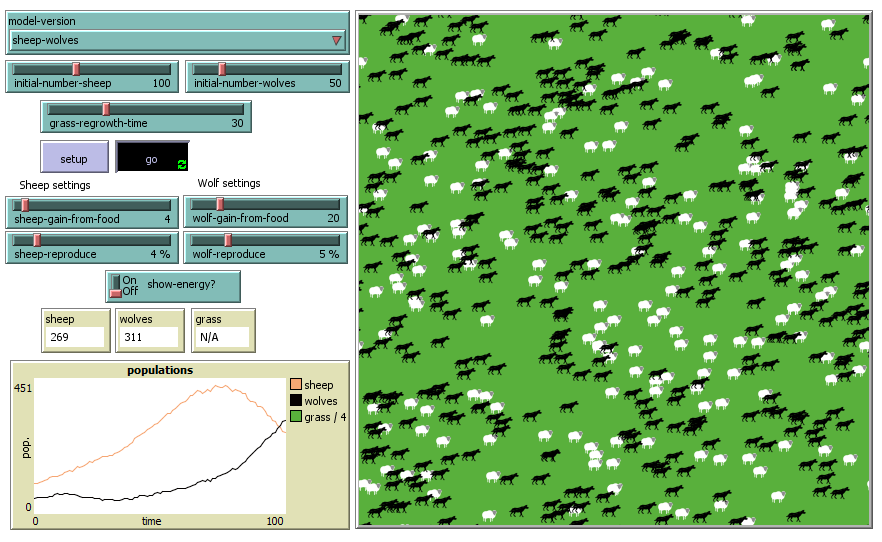
\includegraphics[scale = 0.68]{images/4.png}
	\caption{Демонстрация в режиме sheep-wolfes}
\end{figure}

При нормальной скорости моделирования можно в режиме реального времени наблюдать, количество агентов визуально, а также при помощи графика и полей вывода статистики. 

Заметим, что при заданных параметрах в начале моделирования овцы нескольно теряют свою численность, а волков становится больше, но посмотрим что будет дальше.

\clearpage

\begin{figure}[h!]
	\centering
	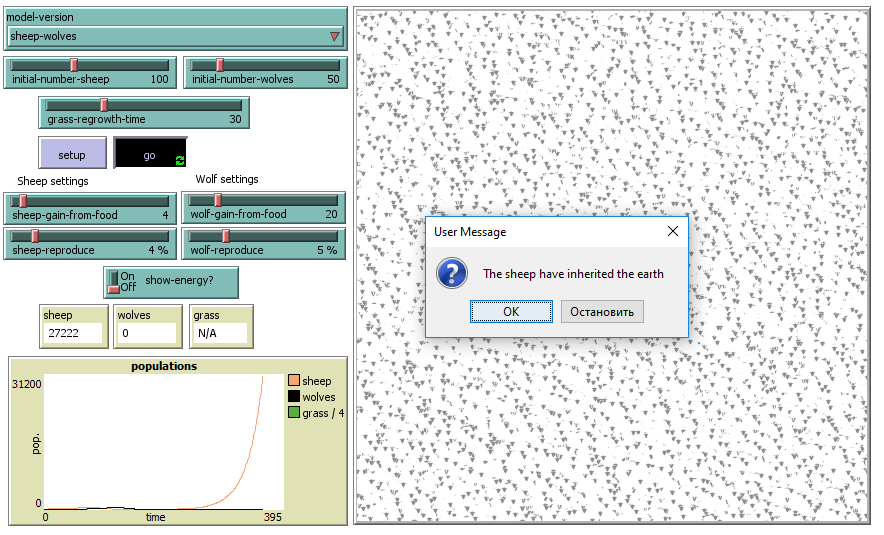
\includegraphics[scale = 0.68]{images/5.png}
	\caption{Результат демонстрации в режиме sheep-wolfes}
\end{figure}

Конец моделирования показал, что овцы бескомпромисно задавили волков по популяции. Из этого можно сделать выводы, что промежуточные результаты не всегда так важны как макрозакономерности, которые такие системы пытаются выявить.

Запустим демонстрационный проект в режиме sheep-wolfes-grass:

\begin{figure}[h!]
	\centering
	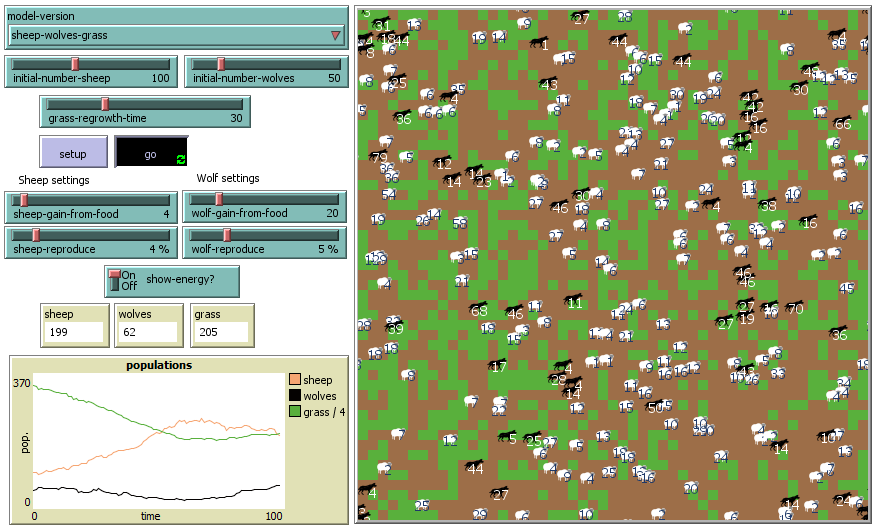
\includegraphics[scale = 0.68]{images/6.png}
	\caption{Демонстрация в режиме sheep-wolfes-grass}
\end{figure}

Как можно заметить по графику данные о популяции овец и травы постепенно изменяются на коротком промежутке времени.

\clearpage

\begin{figure}[h!]
	\centering
	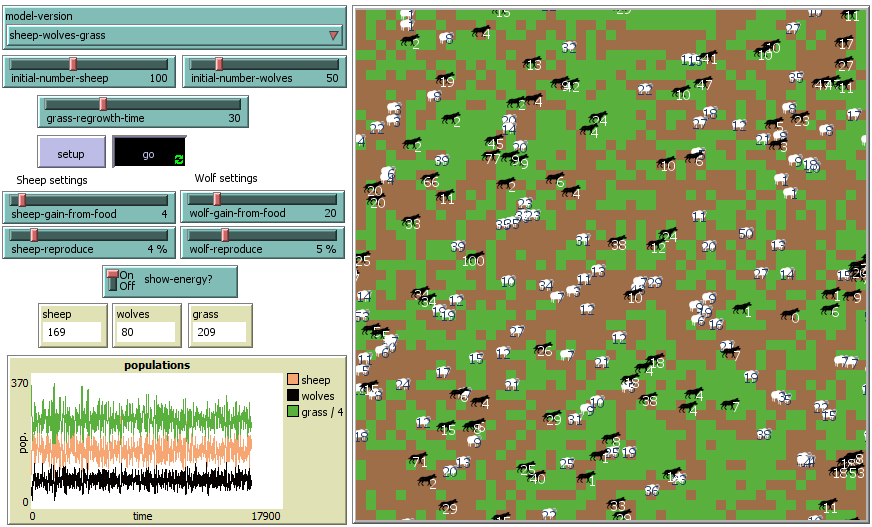
\includegraphics[scale = 0.63]{images/7.png}
	\caption{Результат демонстрации в режиме sheep-wolfes-grass}
\end{figure}

Однако, на большом промежутке времени оказалось, что ни одна из популяций победить не может, они необходимы друг другу для нормального сосуществования. Можно провести аналогию с реальным миром: волки и овцы (хоть и не в изолированной системе) за тысячи лет не уничтожили друг друга.

\subsubsection{Анализ кода}

Код пишется на одноименном языке NetLogo, который является продолжением языка Лого -- первого языка, созданного еще в 1968 году объединенными усилиями Массачусетского Технологического Института и корпорации BBN (Bolt Beranek \& Newman) с целью обучать детей при помощи компьютера [6]

NetLogo является процедурным, агентно-ориентированным языком программирования, который позволяет очень лаконично описывать мультиагентные системы.

Рассмотрим исходный код инициализации агентов:

\lstinputlisting{listings/1.nlogo}

В первую очередь описываются глобальные переменные командами global, breed, turtles-own, ninjas-own. 

Процедуры, в том числе и обслуживающие элементы управления, описываются следующим синтаксисом:

\begin{verbatim}
to setup
    ...
end
\end{verbatim}

Первой операцией процедуры setup является clear-all, которая очищает основной экран. Далее инициализируется константа max-sheep и инициализируются клетки с травой (в зависимости от режима).

После этого инициализируется заданное количество овец (create-sheep) и волков (create-wolf) со случайным показателем энергии и в случайных местах.

Рассмотрим код обработчика такта:

\lstinputlisting{listings/2.nlogo}

В первую очередь выполняется проверка на количество агентов: если все вымерли или стало слишком много, то завершаем работу. После чего вызываются процедуры движения (move) и, в случае совпадения клеток овцы и волка, съедения овцы (eat-ship). Кроме того производится проверка на количество энергии овцы и волка, а также смерть в случае, если она равна нулю (death).

В конце процедуры вызывается процедура прорисовки травы (grow-grass) и инициируется новый такт (tick).

Рассмотрим код используемых процедур:

\lstinputlisting{listings/3.nlogo}

Разбиение кода на независимые процедуры сделало его намного более понятным и простым, хотя и без этого на языке NetLogo подобные сложные системы описываются достаточно просто и интуитивно понятно.

\subsubsection{Опишите основные возможности данного ПО применительно для создания многоагентных систем}

Среда NetLogo является мощной и в то же время интуитивно понятной средой для проектирования многоагентных систем. NetLogo подходит для использования детьми (для которых и была разработана) или же серьезных ученых.

В качестве иллюстрации многогранности решаемых задач, приведем еще пару примеров:

\begin{figure}[h!]
	\centering
	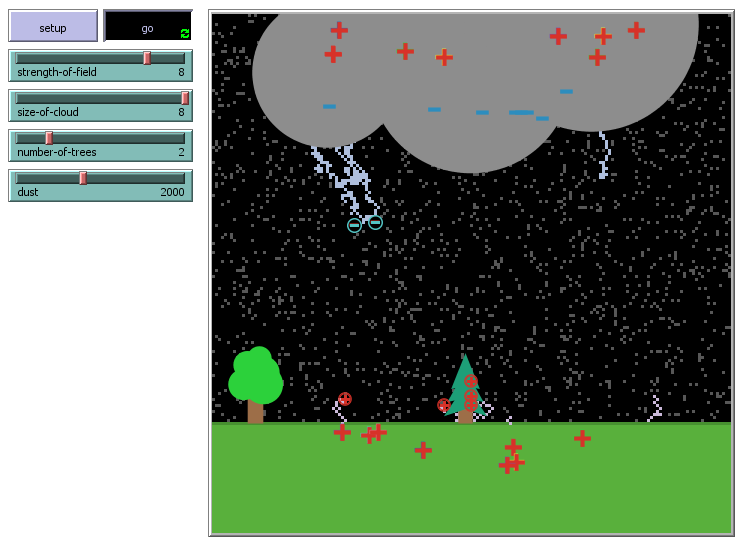
\includegraphics[scale = 0.49]{images/8.png}
	\caption{Моделирование процесса создания молнии}
\end{figure}

\begin{figure}[h!]
	\centering
	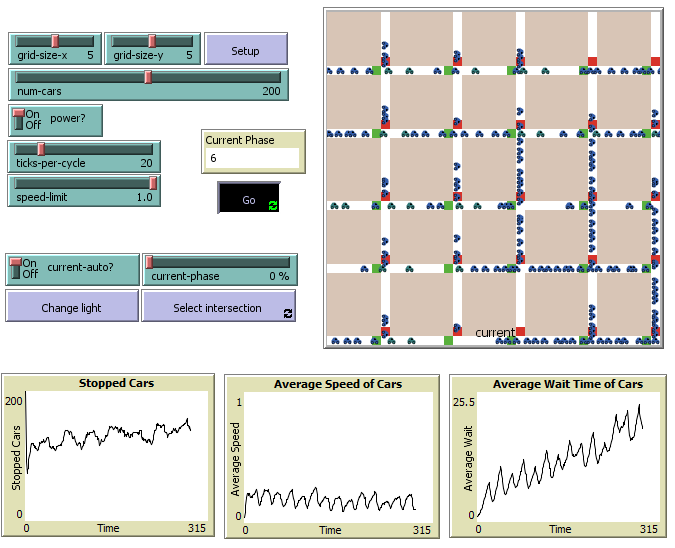
\includegraphics[scale = 0.49]{images/9.png}
	\caption{Анализ дорожной ситуации на возникновение пробок}
\end{figure}

Таким образом NetLogo может быть использована для самого широкого спектра многоагентных задач, от анализа дорожной ситуации до компьютерных игр.

\section{Вывод}

В ходе работы были изучены принципы работы многоагентных систем. Был произведен анализ преимуществ и недостатков данного подхода, рассмотрена классификация, а также изучена среда для разработки многоагентных систем NetLogo.

\subsubsection{В чем Плюсы и минусы многоагентного подхода?}

Основные преимущества использования многоагентных систем, это: \textbf{распределенные вычисления}, \textbf{масштабирование} и \textbf{автономность}. Кроме того агенты могут общаться между собой, обмениваться информацией и кооперироваться для выполнения задач.

Из недостатков следует выделить усложнение структуры за счет количества агентов, что впоследствии ведет к \textbf{плохой наблюдаемости} и \textbf{непредсказуемости} системы.

\subsubsection{Какие еще среды или языки программирования использует для создания многоагентных систем?}

Для разработки многоагентных системы наилучшим образом подойдут следующие программные средства: Python, Matlab, Logo, NetLogo, StarLogo, Kiva, Repast Simphony, Eclipse AMP, JADE, Jason.

\subsubsection{Как по-вашему стоит ли развивать данное направление, если нет, то почему, если да, то в какую сторону?}

При наличии достаточных вычислительных мощностей было бы здорово увидеть многоагентную систему моделирования работы нейронов головного мозга.

Кроме того, такие системы великолепно подходят для выявления макрозакономерностей в таких важнейших науках, как биолгия, физика, химия, социология и др. Поэтому нужно продолжать двигаться в этом направлении и постепенно увеличивать наши знания о мире.

\subsubsection{Корректно ли по-вашему моделирование многоагентных систем на одной вычислительной машине?}

Как и для любого программного средства, ответ на этот вопрос зависит от сложности задачи. Для простой многоагентной системы вполне достаточно и одного компьютера.

\subsubsection{Приведите области в которых применение многоагентного подхода дает максимально положительные результаты.}

\begin{itemize}
	\item Выявление макрозакономерностей в естественных науках и социальных исследованиях.
	\item Исследование нагруженности сетевых и мобильных сервисов.
	\item Исследование предпочтений пользователей.
	\item Доказательство математических теорем.
\end{itemize}

\clearpage

\section{Список литературы}

\begin{flushleft}
	
[1] Многоагентные системы AI Portal [Электронный ресурс]. — URL: \href{http://www.aiportal.ru/articles/multiagent-systems/multiagent-systems.html}{http://www.aiportal.ru/articles/multiagent-systems/multiagent-systems.html} (дата обращения 25.11.2017). \linebreak
	
[2] ИНТЕЛЛЕКТУАЛЬНЫЕ МИКРОРОБОТОТЕХНИЧЕСКИЕ АГЕНТЫ И МНОГОАГЕНТНЫЕ МИКРОСИСТЕМЫ [Электронный ресурс]. — URL: \href{http://www.microsystems.ru/files/publ/205.htm}{http://www.microsystems.ru/files/publ/205.htm} (дата обращения 25.11.2017). \linebreak

[3] Агенты, многоагентные системы, виртуальные [Электронный ресурс]. — URL: \href{http://pandia.ru/text/78/362/252-2.php}{http://pandia.ru/text/78/362/252-2.php} (дата обращения 25.11.2017). \linebreak

[4] Мультиагентные системы [Электронный ресурс]. — URL: \href{http://mabi.vspu.ru/portfolio/multiagentnyie-sistemyi/}{http://mabi.vspu.ru/portfolio/multiagentnyie-sistemyi/} (дата обращения 25.11.2017). \linebreak

[5] Классификация агентов [Электронный ресурс]. — URL: \href{http://www.aiportal.ru/articles/multiagent-systems/agent-classification.html}{http://www.aiportal.ru/articles/multiagent-systems/agent-classification.html} (дата обращения 25.11.2017). \linebreak

[6] NetLogo Letopisi [Электронный ресурс]. — URL: \href{http://letopisi.org/index.php/NetLogo}{http://letopisi.org/index.php/NetLogo} (дата обращения 25.11.2017). \linebreak

[7] Download NetLogo [Электронный ресурс]. — URL: \href{https://ccl.northwestern.edu/netlogo/download.shtml}{https://ccl.northwestern.edu/netlogo/download.shtml} (дата обращения 25.11.2017). \linebreak

\end{flushleft}
	


\end{document}